\chapter{Tag 17 — Große Codes und Interleaving}

\begin{quote}
Bisher konntest du Datamatrix-Symbole bis 26×26 kodieren und wieder
dekodieren. In der echten Welt — auf Pharmapackungen, Bauteilbändern,
Versandlabeln — gehen die Symbole bis 144×144 und tragen mehrere hundert
Datenbytes. Das bringt ein neues Problem: Was passiert, wenn ein
Kratzer quer über das Symbol geht?
\end{quote}

\section*{Lernziele für heute}

Am Ende von Tag 17 kannst du \dots

\begin{itemize}
\item erklären, warum ein einzelner RS-Block bei großen Symbolen
  gegen lokale Beschädigungen verwundbar ist
\item das Interleaving-Prinzip beschreiben: Daten auf mehrere
  RS-Blöcke aufteilen und die Codewords verschachteln
\item \texttt{teile\_in\_bloecke} und \texttt{verschachtle\_bloecke}
  implementieren und mit Bleistift nachvollziehen
\item die \texttt{DatamatrixEncoderGross}-Klasse einsetzen, um
  Symbole bis 64×64 zu erzeugen
\end{itemize}

\paragraph{Material} Laptop mit Thonny, \texttt{reedsolo} und
\texttt{pylibdmtx} aus den Vortagen.

% =============================================================
\section{Das Kratzer-Problem \normalfont(\textit{≈ 10 min})}
% =============================================================

Stell dir ein 144×144-Datamatrix-Symbol auf einem Pharmakarton vor.
Der Karton rutscht über einen Tisch und bekommt einen Kratzer quer
über das ganze Symbol — eine horizontale Linie, die 10 Zeilen von
Modulen unlesbar macht.

\textbf{Ohne Interleaving} liegen alle Codewords sequenziell in der
Matrix. Die 10 zerstörten Zeilen enthalten lauter aufeinander­folgende
Codewords — aus demselben RS-Block. Wenn das 30 Codewords auf einmal
sind und der Block nur 20 korrigieren kann, ist das Symbol verloren.

\textbf{Mit Interleaving} werden die Codewords auf mehrere RS-Blöcke
aufgeteilt und verschachtelt in die Matrix geschrieben. Codeword~1
gehört Block~1, Codeword~2 zu Block~2, Codeword~3 wieder Block~1 usw.
Dieselben 10 zerstörten Zeilen treffen jetzt \emph{jeden Block gleich
oft} — jeder Block verliert nur einen Bruchteil seiner Codewords und
kann sich selbst reparieren.

\begin{center}
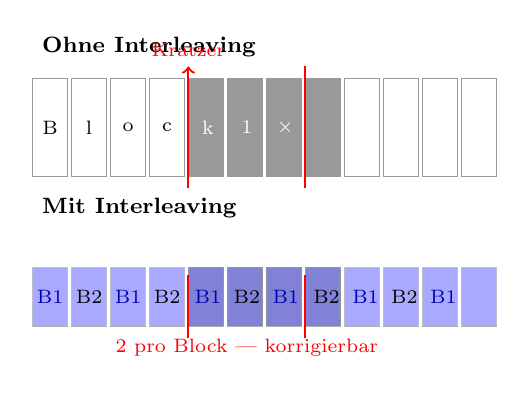
\begin{tikzpicture}[x=0.45cm, y=0.5cm, font=\footnotesize]
  % Ohne Interleaving — ein Block
  \node[anchor=west] at (0, 3.3) {\textbf{Ohne Interleaving}};
  \foreach \i in {0,...,11} {
    \pgfmathtruncatemacro{\shade}{(\i > 3 && \i < 8) ? 40 : 0}
    \fill[black!\shade!white, draw=black!40, thin]
      (\i*1.1, 0) rectangle ++(1, 2.5);
  }
  \node[font=\scriptsize] at (0.5, 1.25)  {B};
  \node[font=\scriptsize] at (1.6, 1.25)  {l};
  \node[font=\scriptsize] at (2.7, 1.25)  {o};
  \node[font=\scriptsize] at (3.8, 1.25)  {c};
  \node[font=\scriptsize, white] at (4.95, 1.25) {k};
  \node[font=\scriptsize, white] at (6.05, 1.25) {1};
  \node[font=\scriptsize, white] at (7.15, 1.25) {×};
  \node[font=\scriptsize] at (8.3, 1.25)  {};
  \draw[red, thick, ->] (4.4, -0.3) -- (4.4, 2.8)
    node[above, red, font=\scriptsize] {Kratzer};
  \draw[red, thick] (7.7, -0.3) -- (7.7, 2.8);
  % Mit Interleaving — zwei Blöcke abwechselnd
  \node[anchor=west] at (0, -0.8) {\textbf{Mit Interleaving}};
  \foreach \i in {0,...,11} {
    \pgfmathtruncatemacro{\shade}{(\i > 3 && \i < 8) ? 40 : 0}
    \pgfmathtruncatemacro{\isB}{\i - 2*(\i/2)}  % mod 2 approx
    \pgfmathtruncatemacro{\col}{(\isB == 0) ? 70 : 0}
    \fill[blue!\col!white, draw=black!40, thin, opacity=0.8]
      (\i*1.1, -3.8) rectangle ++(1, 1.5);
    \fill[black!\shade!white, draw=none, opacity=0.4]
      (\i*1.1, -3.8) rectangle ++(1, 1.5);
  }
  \node[font=\scriptsize, blue!70!black] at (0.5,  -3.05) {B1};
  \node[font=\scriptsize]               at (1.6,  -3.05) {B2};
  \node[font=\scriptsize, blue!70!black] at (2.7,  -3.05) {B1};
  \node[font=\scriptsize]               at (3.8,  -3.05) {B2};
  \node[font=\scriptsize, blue!70!black] at (4.95, -3.05) {B1};
  \node[font=\scriptsize]               at (6.05, -3.05) {B2};
  \node[font=\scriptsize, blue!70!black] at (7.15, -3.05) {B1};
  \node[font=\scriptsize]               at (8.3,  -3.05) {B2};
  \node[font=\scriptsize, blue!70!black] at (9.4,  -3.05) {B1};
  \node[font=\scriptsize]               at (10.5, -3.05) {B2};
  \node[font=\scriptsize, blue!70!black] at (11.6, -3.05) {B1};
  \draw[red, thick] (4.4, -4.1) -- (4.4, -2.5);
  \draw[red, thick] (7.7, -4.1) -- (7.7, -2.5);
  \node[font=\scriptsize, red] at (6.05, -4.35) {2 pro Block — korrigierbar};
\end{tikzpicture}
\end{center}

Das 36×36-Symbol links ist sauber; beim rechten hat ein horizontaler
Kratzer einige Datenmodule zerstört. Weil die Codewords verschachtelt
sind, trifft der Kratzer beide RS-Blöcke je einmal — jeder Block
repariert sich selbst.

\begin{center}
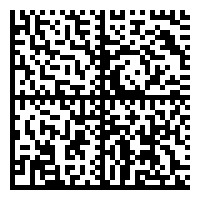
\includegraphics[width=0.32\linewidth]{abbildungen/tag17/interleaving_36x36_sauber.png}
\hspace{1cm}
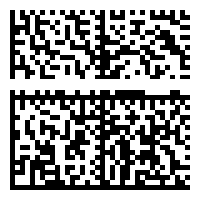
\includegraphics[width=0.32\linewidth]{abbildungen/tag17/interleaving_36x36_kratzer_klein.png}
\end{center}

% =============================================================
\section{Wie Interleaving funktioniert \normalfont(\textit{≈ 15 min})}
% =============================================================

Die Tabelle unten zeigt, welche Symbole mehrere RS-Blöcke nutzen.
Ab 36×36 (2×2 Datenbereiche im Symbol) gibt es 2 RS-Blöcke:

\begin{center}
\begin{tabular}{lrrrl}
\toprule
Größe & Daten-CW & ECC-CW & RS-Blöcke & Zeichenkapazität \\
\midrule
26×26 &  44 &  28 & 1 &  44 Zeichen \\
32×32 &  62 &  50 & 1 &  62 Zeichen \\
\midrule
36×36 &  86 &  42 & 2 &  86 Zeichen \\
40×40 & 114 &  46 & 2 & 114 Zeichen \\
44×44 & 144 &  56 & 2 & 144 Zeichen \\
48×48 & 174 &  66 & 2 & 174 Zeichen \\
52×52 & 204 &  84 & 2 & 204 Zeichen \\
\bottomrule
\end{tabular}
\end{center}

Der Ablauf für ein 36×36-Symbol (\texttt{k=2}):

\begin{enumerate}
\item \textbf{Aufteilen}: die 86 gepadde\-ten Datenbytes werden in
  2 Blöcke geteilt — Block~1 bekommt 43 Bytes, Block~2 ebenfalls 43.
\item \textbf{ECC pro Block}: für jeden Block werden separat 21 ECC-Bytes
  berechnet (insgesamt 42 ECC-Bytes, wie in der Tabelle).
\item \textbf{Verschachteln}: die finale Codeword-Sequenz entsteht
  durch round-robin-Mischen. Zuerst die Datenbytes:
  D1[0], D2[0], D1[1], D2[1], \ldots\ dann die ECC-Bytes:
  E1[0], E2[0], E1[1], E2[1], \ldots

\end{enumerate}

\begin{bleistiftuebung}{1}{Interleaving von Hand}
Gegeben: 6~Datenbytes \texttt{[A, B, C, D, E, F]}
(\texttt{A}=65 usw.) und \texttt{k=2} Blöcke mit je 3~ECC-Bytes.

\begin{enumerate}
\item Teile die 6 Bytes auf 2 Blöcke auf. Welche Bytes sind in Block~1,
  welche in Block~2?
\item Stell dir vor, die ECC-Bytes für Block~1 sind \texttt{[p, q, r]}
  und für Block~2 \texttt{[s, t, u]}. Wie sieht die verschachtelte
  Codeword-Sequenz aus?
\item Welche Codewords würden durch einen Kratzer, der die Positionen
  3, 4 und 5 trifft, zerstört? Treffen sie Block~1, Block~2 oder beide?
\end{enumerate}

Tipp: schreib die Sequenz aus Schritt 2 als Liste auf.
\end{bleistiftuebung}

% =============================================================
\section{Python-Umsetzung \normalfont(\textit{≈ 30 min})}
% =============================================================

\begin{pythoneinheit}{1}{Hilfsfunktionen: aufteilen und verschachteln}
\pythoncodeteil{tag17/interleaving.py}{bloecke}

Drei Funktionen — drei Schritte:

\begin{itemize}
\item \texttt{teile\_in\_bloecke(codewords, k)} teilt eine Liste möglichst
  gleichmäßig auf. Ist die Länge nicht durch~\texttt{k} teilbar, bekommt
  der erste Block ein Byte mehr.
\item \texttt{reed\_solomon\_pro\_block} nutzt \texttt{reedsolo} genau
  wie in Etappe~8 und 16 — dieselben Parameter \texttt{prim=0x12D,
  fcr=1, generator=2}. Jeder Block wird \emph{unabhängig} kodiert.
\item \texttt{verschachtle\_bloecke} mischt zuerst die Datenbytes
  round-robin, dann die ECC-Bytes. Das ist die Codeword-Sequenz, die
  in die Matrix gehen würde.
\end{itemize}
\end{pythoneinheit}

\begin{pythoneinheit}{2}{Erweiterte Symbol-Tabelle}
\pythoncodeteil{tag17/interleaving.py}{tabelle}

Der dritte Eintrag pro Zeile ist die Anzahl der RS-Blöcke. Für kleine
Symbole (bis 32×32) bleibt es bei einem Block — der bisherige
\texttt{DatamatrixEncoder} funktioniert weiter unverändert. Ab 36×36
kommen 2 Blöcke, weil das Symbol dann intern aus vier
Datenbereichen (2×2-Gitter) besteht, die je eigene Ausrichtungs\-muster
haben.
\end{pythoneinheit}

\begin{pythoneinheit}{3}{\texttt{DatamatrixEncoderGross} — Subklasse mit Interleaving}
\pythoncodeteil{tag17/encoder_gross.py}{klasse}

Die Subklasse überschreibt zwei Klassenvariablen und den Konstruktor:

\begin{itemize}
\item \texttt{SYMBOL\_TABLE} wird auf das vollständige 2-Tupel-Format
  des Eltern-Encoders gebracht (ohne Block-Anzahl — die braucht
  \texttt{DatamatrixEncoder} nicht).
\item \texttt{\_RS\_BLOECKE} ist ein privates Dict nur für diese Klasse.
\item Im Konstruktor: Ist \texttt{k=1}, werden Padding und ECC direkt
  von der Elternklasse erledigt. Für \texttt{k>1} greifen unsere
  drei Hilfsfunktionen.
\item \texttt{save\_png()} delegiert das Rendering großer Symbole an
  \texttt{pylibdmtx} — die Daten­platzierung in Multi-Bereich-Symbolen
  ist zu aufwändig, um sie selbst zu bauen.
\end{itemize}
\end{pythoneinheit}

\begin{pythoneinheit}{4}{Demo: kleines und großes Symbol}
\pythoncodeteil{tag17/encoder_gross.py}{demo}

Erwartete Konsolenausgabe:

\begin{minted}{text}
DatamatrixEncoderGross(text='GRETA', 12×12, 5+7 CW, 1 RS-Block)
  Scan: GRETA

DatamatrixEncoderGross(text='INTERLEAVING VERTEILT ...', 36×36,
  86+42 CW, 2 RS-Blocke)
  Scan: INTERLEAVING VERTEILT SCHAEDEN AUF MEHRERE RS-BLOECKE
  Codewords (erste 10): [74, 83, 79, 84, 85, 46, 70, 67, 83, 77]
\end{minted}

Das 36×36-Symbol scannt korrekt — das beweist, dass unsere
Codeword-Berechnung mit der von \texttt{pylibdmtx} übereinstimmt
(gleicher Standard, gleiche Parameter).

Zur Erinnerung: aus Etappe~16 haben wir den \texttt{DatamatrixDecoder}
mit Fehlermarkierung. Links das 12×12-Symbol mit drei zufällig
geflippten Modulen; rechts alle Module der betroffenen Codewords
rot markiert — trotzdem \textbf{erfolgreich dekodiert}.

\begin{center}

\includegraphics[width=0.28\linewidth]{abbildungen/tag17/greta_12x12_kaputt.png}
\hspace{1.5cm}

\includegraphics[width=0.28\linewidth]{abbildungen/tag17/greta_12x12_markiert.png}
\end{center}
\end{pythoneinheit}

\begin{bleistiftuebung}{2}{Eigenen Text in 36×36}
Wähle einen eigenen Text, der zwischen 44 und 86 Zeichen lang ist
(damit er für 36×36 qualifiziert, aber nicht in 26×26 passt). Tipp:
Deinen vollen Namen + Geburtsdatum. Enkodiere ihn mit
\texttt{DatamatrixEncoderGross(dein\_text, n=36)} und prüfe mit deinem
Handy, ob das Symbol scannt. Wie viele Bytes landen in Block~1,
wie viele in Block~2?
\end{bleistiftuebung}

% =============================================================
\section{Reflexion und Brücke zu Tag 18 \normalfont(\textit{≈ 10 min})}
% =============================================================

Du hast heute gelernt:

\begin{itemize}
\item Ohne Interleaving ist ein großes Symbol anfällig für Kratzer:
  ein lokaler Schaden häuft Fehler in einem RS-Block — der bricht.
\item Mit Interleaving wird der Schaden auf alle Blöcke verteilt.
  Jeder Block erholt sich selbst — klassische „Teile und herrsche"-Idee.
\item Die Grenze ist nicht willkürlich: ab 36×36 hat das Symbol
  mehrere physische Datenbereiche mit eigenen Ausrichtungs­mustern.
  Die Block-Anzahl folgt aus der Symbolstruktur.
\item Das Rendering großer Symbole haben wir an \texttt{pylibdmtx}
  übergeben. Das ist keine Niederlage — es ist gutes Software-Design:
  nutze erprobte Bibliotheken für komplexe, aber bekannte Probleme.
\end{itemize}

\subsection*{Vorschau Tag 18}

Wir haben bisher immer reinen Großbuchstaben-Text kodiert, der
zeichenweise in einem Byte landet. Aber Datamatrix hat noch mehr
Kodierungs­modi:

\begin{itemize}
\item \textbf{ASCII-Modus} (den wir nutzen): 1 Byte pro Zeichen
\item \textbf{Digit-Paar-Modus}: zwei Ziffern in einem Byte —
  damit passen doppelt so viele Zahlen in dasselbe Symbol
\item \textbf{C40-Modus}: drei Großbuchstaben in zwei Bytes —
  effizienter für alphanumerische Texte
\end{itemize}

Wir schauen uns an, wie der Encoder erkennt, welcher Modus gerade
am effizientesten ist, und bauen einen einfachen automatischen
Moduswechsler.
